\documentclass[12pt,letterpaper]{article}
\usepackage[utf8]{inputenc}
\usepackage[T1]{fontenc}
\usepackage[spanish]{babel}
\usepackage{geometry}
\usepackage{graphicx}
\usepackage{longtable}
\usepackage{hyperref}
\geometry{margin=2.2cm}
\title{Robot Minisumo}
\author{Álvarez Villegas José Ángel\\MICROCONTROLADORES\\Grupo 2809}
\date{2026-06-05}
\begin{document}
\maketitle
\tableofcontents
\newpage
\section{Introducción}
El Robot Minisumo es un prototipo autónomo basado en Arduino Nano, sensores TCRT5000, HC-SR04, buzzer KY-012 y servomotores SG90.
\section{Objetivo general}
Consolidar un prototipo funcional con documentación, firmware, validación, esquemático KiCad y entregables finales.
\section{Materiales y equipo}
La BOM final se documenta en \texttt{docs/bom\_final.md} y \texttt{report/assets/bom\_final.md}.
\section{Lista final de conexiones}
\begin{longtable}{p{4cm}p{3cm}p{3cm}p{4cm}}
\textbf{Componente} & \textbf{Pin componente} & \textbf{Pin Arduino} & \textbf{Señal}\\
TCRT5000 Left & DO & D3 & TCRT\_LEFT \\
TCRT5000 Right & DO & D2 & TCRT\_RIGHT \\
TCRT5000 Back & DO & D0 & TCRT\_BACK \\
HC-SR04 & Trig & D4 & TRIG\_HCSR04 \\
HC-SR04 & Echo & D5 & ECHO\_HCSR04 \\
KY-012 & S & D7 & BUZZER\_SIG \\
SG90 Left & Signal & D9 & SERVO\_LEFT \\
SG90 Right & Signal & D10 & SERVO\_RIGHT \\
\end{longtable}
\textbf{Advertencia:} D0 y D1 corresponden a RX/TX del Arduino Nano. El prototipo final usa D0 para TCRT Back, por lo que puede ser necesario desconectarlo durante carga de firmware.
\section{Diagrama final de conexiones}
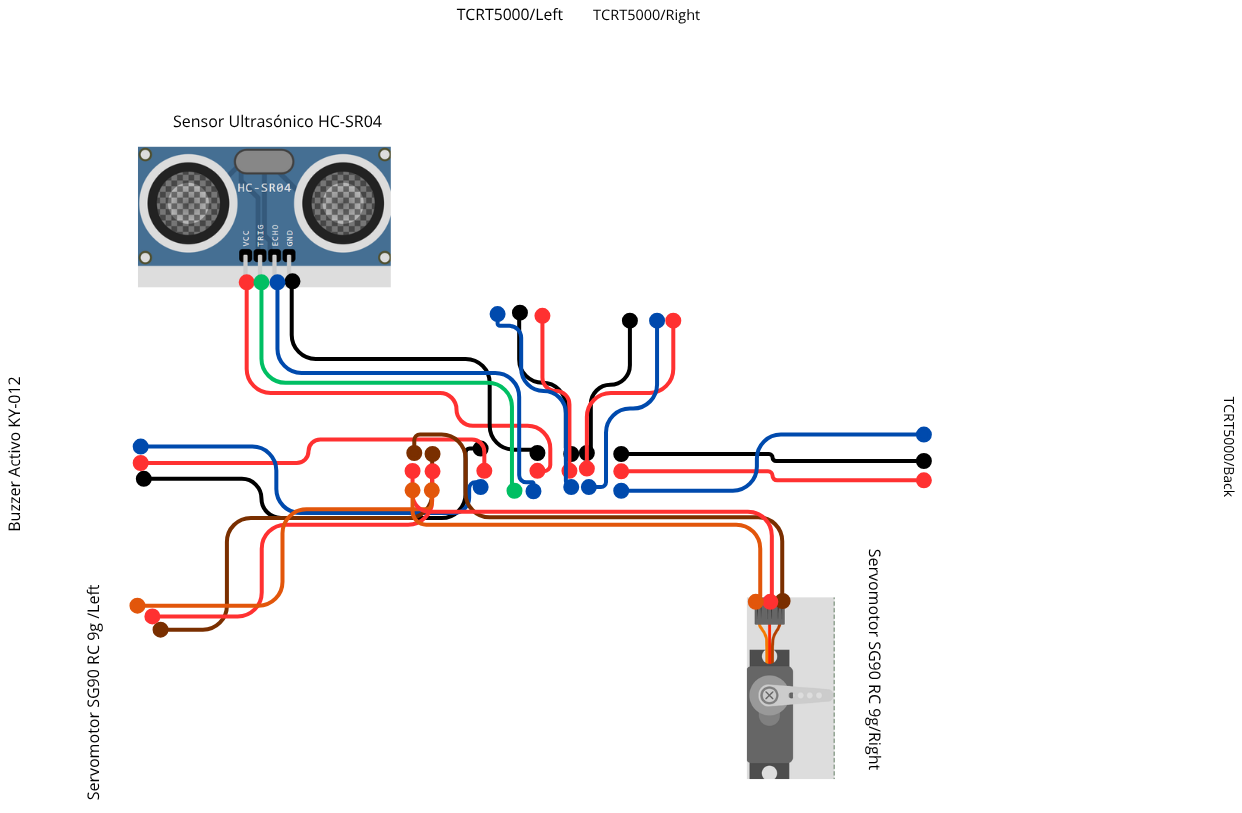
\includegraphics[width=\textwidth]{assets/diagrama_conexiones_final.png}
Version PDF del diagrama final: \texttt{assets/diagrama\_conexiones\_final.pdf}.
\section{Funcionamiento}
El robot prioriza la evasión de borde; si no hay borde, mide distancia y ataca cuando el oponente está a 35 cm o menos. Si no detecta oponente, busca girando.
\section{Código implementado}
El firmware final se encuentra en \texttt{firmware/robot\_minisumo\_final/robot\_minisumo\_final.ino} e incluye funciones modulares de lectura, movimiento, ataque, búsqueda, evasión y pruebas.
\section{Pseudocódigo y diagramas}
Ver \texttt{docs/pseudocodigo.md} y \texttt{docs/diagramas\_flujo.md}.
\section{Simulación y validación}
La validación se documenta por casos en \texttt{simulation/casos\_prueba.md}.
\section{Pruebas realizadas}
\begin{longtable}{p{9cm}p{5cm}}
\textbf{Prueba} & \textbf{Estado}\\
Buzzer KY-012 & Aprobado \\
HC-SR04 & Aprobado \\
TCRT5000 Left & Aprobado \\
TCRT5000 Right & Aprobado \\
TCRT5000 Back & Aprobado \\
Servo D9 aislado & Aprobado \\
Servos D9/D10 conjunto & Aprobado \\
Firmware final & Aprobado \\
Robot fisico & Aprobado \\
\end{longtable}
\section{Evidencia del prototipo funcional}
La evidencia multimedia del prototipo funcional se organizo en \texttt{assets/} y se documento en \texttt{docs/evidencia\_multimedia.md}, \texttt{docs/inventario\_multimedia.md} y \texttt{validation/evidencia\_funcionamiento.md}.

\begin{longtable}{p{5cm}p{5cm}p{4cm}}
\textbf{Evidencia} & \textbf{Archivo} & \textbf{Utilidad}\\
Diagrama final & \texttt{assets/images/conexiones/robot\_minisumo\_conexiones\_diagrama\_final\_01.png} & Pinout real del robot. \\
Montaje frontal & \texttt{assets/robot\_minisumo\_montaje\_frontal\_hcsr04\_01.jpg} & HC-SR04 al frente del prototipo. \\
Montaje posterior & \texttt{assets/robot\_minisumo\_montaje\_posterior\_electronica\_01.jpg} & Arduino Nano, shield, buzzer y cableado. \\
Panel web & \texttt{assets/robot\_minisumo\_panel\_monitoreo\_desktop\_01.png} & Panel minimalista usado durante la grabacion. \\
Video final & \texttt{assets/videos/demo\_final/robot\_minisumo\_demo\_funcionamiento\_final\_01.mp4} & Demostracion del robot funcionando. \\
\end{longtable}

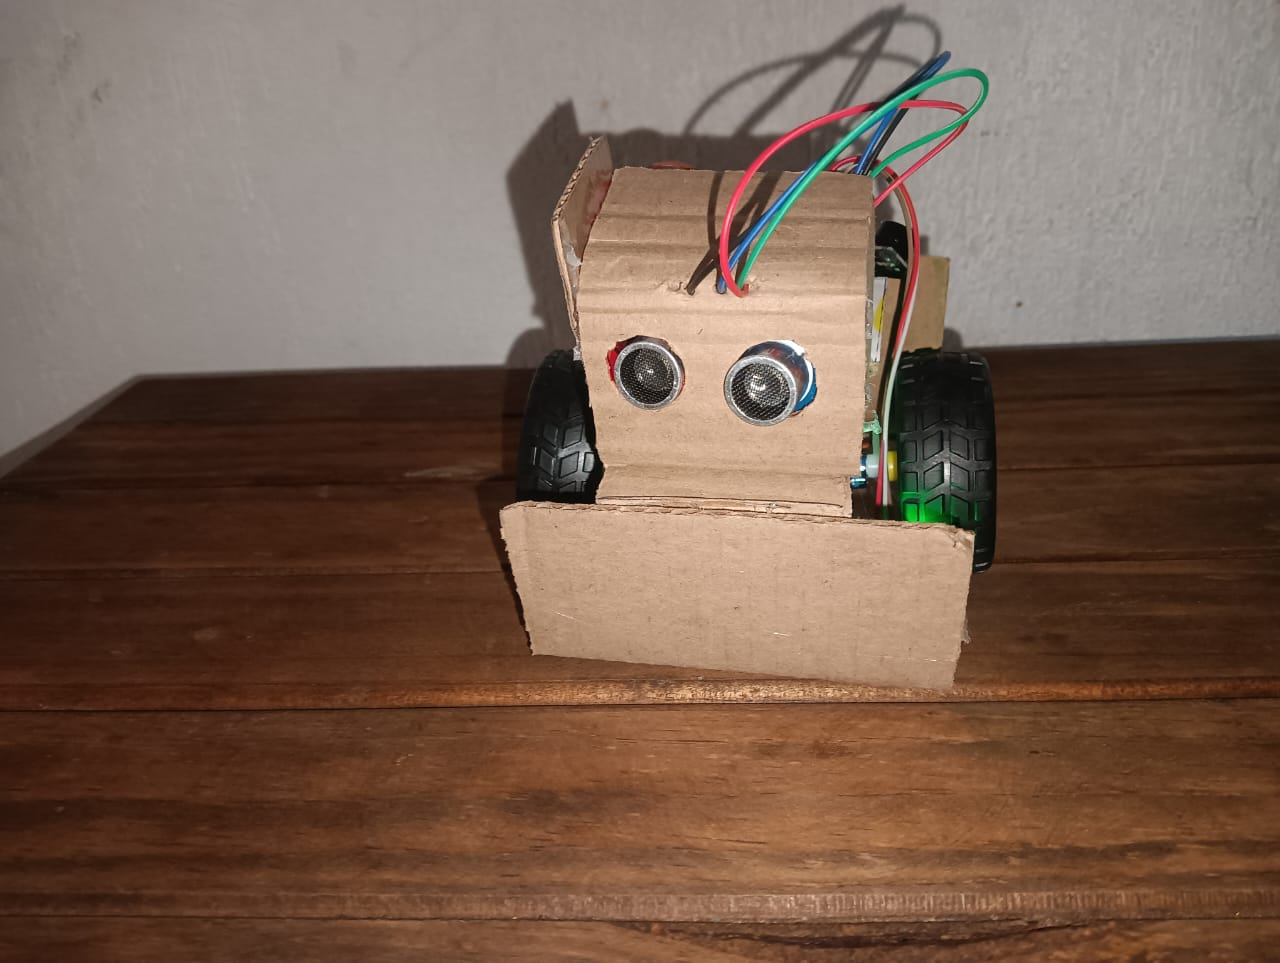
\includegraphics[width=0.82\textwidth]{assets/robot_minisumo_montaje_frontal_hcsr04_01.jpg}

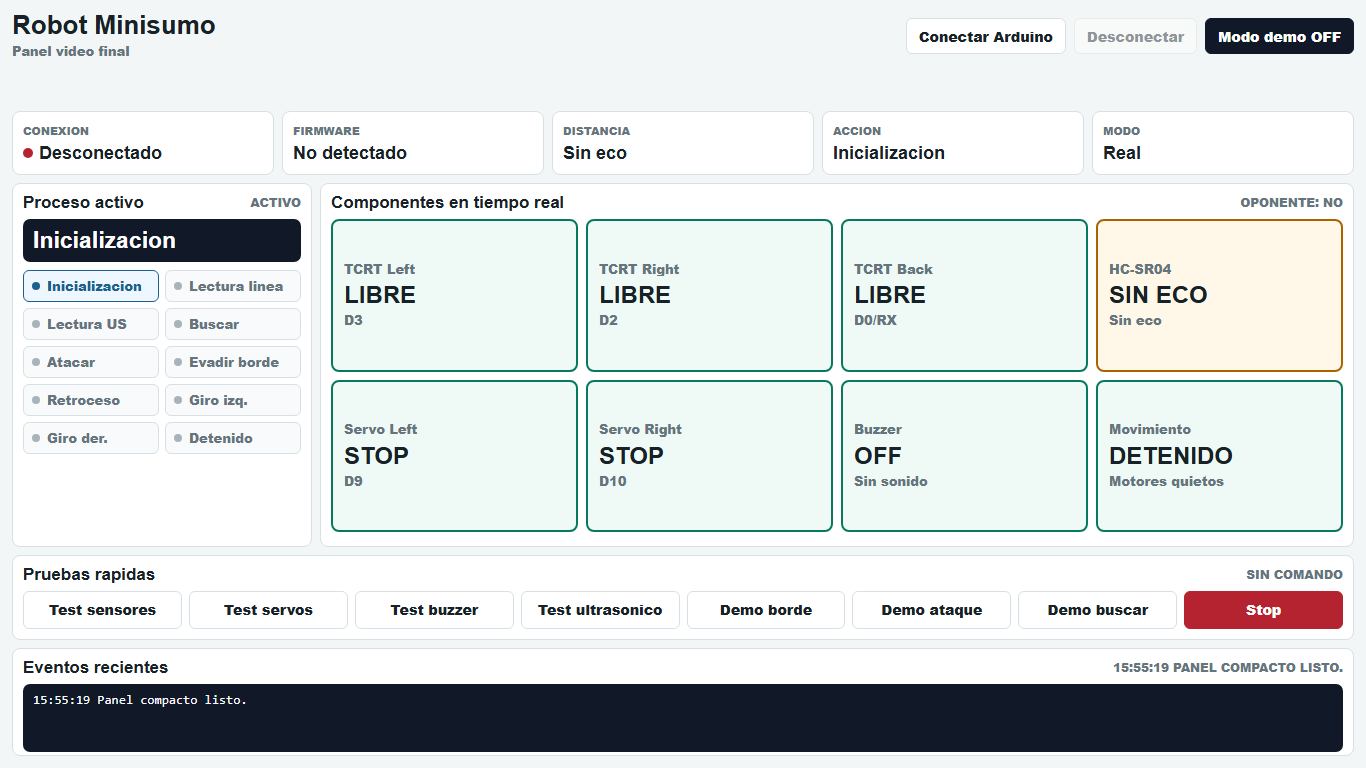
\includegraphics[width=\textwidth]{assets/robot_minisumo_panel_monitoreo_desktop_01.png}

Los videos incluidos son ligeros para publicacion en GitHub; el archivo mas grande pesa 3.39 MB, por lo que no se uso Git LFS.

\\section{Resultados}
El prototipo físico se encuentra funcional. Se confirmaron sensores, buzzer y servos SG90 con el pinout final real.
\section{Conclusiones}
El proyecto queda listo para entrega académica y publicación técnica. El principal cuidado operativo es el uso de D0/RX para TCRT Back.
\section{Referencias}
Arduino Nano, HC-SR04, TCRT5000, SG90, KY-012, KiCad y documentación generada del proyecto.
\end{document}
